\section{Uniform sampling of the integers}\label{sec:natural}
Let $\delta_z$ be unit point mass at $z$. The empirical law obtained by
giving every integer equal weight is
$\mu_N=N^{-1}\sum_{n=1}^N\delta_{R_{p,q}(n)}$.
Write $\theta_N=\omega\log N\bmod\mathbb Z^2$.
\begin{theorem}\label{thm:natural}
Let $D$ be exponential with mean one. Whenever $N_i\to\infty$ and
$\theta_{N_i}\to\theta$ on $\T^2$,
\[
 \mu_{N_i}\ \Longrightarrow\ \nu_\theta
   :=\Law\!\left(F(\theta-\omega D)\right).
\]
The set of all weak subsequential limits is
$\{\nu_\theta:\theta\in\T^2\}$. The means of these laws vary with
$\theta$, so the full sequence $\mu_N$ has no weak limit.
\end{theorem}
\begin{proof}
For a continuous test function $\varphi$ put $G=\varphi\circ F$.
The identity $\log n=\log N+\log(n/N)$ gives
\[
 \int\varphi\dd\mu_N=\frac1N\sum_{n=1}^N
 G(\theta_N+\omega\log(n/N)).
\]
On $[\delta,1]$, for any $\delta>0$, the summands as functions of $n/N$
converge uniformly along the stated subsequence to
$G(\theta+\omega\log y)$. Ordinary Riemann sums converge there.
The part $n/N<\delta$ contributes at most $\delta\|G\|_\infty$.
Letting $\delta\downarrow0$ and setting $y=e^{-u}$ gives
\begin{equation}
 \int\varphi\dd\nu_\theta=
 \int_0^\infty G(\theta-\omega u)e^{-u}\dd u. \label{eq:natural}
\end{equation}
For each $\theta$ equidistribution supplies $t_i\to\infty$ with
$\omega t_i\to\theta$ modulo $\mathbb Z^2$. Then
$N_i=\lfloor e^{t_i}\rfloor$ satisfies $\log N_i-t_i\to0$.
Conversely compactness gives a convergent phase subsequence from
any subsequence of integers, proving the assertion about all limits.

To distinguish at least two laws, take $\varphi(y)=y$ and write
$H(\theta)=\int y\dd\nu_\theta(y)$. On the torus, \eqref{eq:natural}
gives
\[
 \widehat H(k)=\frac{\widehat F(k)}{1+2\pi i\,k\cdot\omega},\qquad
 \widehat F(k)=\int_{\T^2}F(v)e^{-2\pi i k\cdot v}\dd v .
\]
Indeed this follows by translating the inner integral and applying
Fubini's theorem. For $k=(1,0)$ the numerator is
\[
 \widehat f_p(1)=
 \frac{\ell_p}{\ell_p-2\pi i}+\frac{\ell_p}{2\pi i}
 =\frac{\ell_p^2}{(2\pi i)(\ell_p-2\pi i)}\ne0.
\]
Thus the continuous mean $H$ is nonconstant.
\end{proof}
There is also an integer version of \eqref{eq:loglaw}. Give $n\leq N$
weight $1/(nH_N)$, where $H_N=\sum_{n\leq N}1/n$. For
$G=\varphi\circ F$, the oscillation of $G(\omega\log x)$ on
$[n,n+1]$ tends to zero by uniform continuity. Replacing the
integrand on each interval by its left endpoint therefore costs
$o(\log N)$ in the logarithmic integral. Replacing
$\log(1+1/n)$ by $1/n$ costs $O(1)$ in total. Since
$H_N\sim\log N$, this discrete average has the law of Theorem~\ref{thm:log}.

\begin{figure}[tbp]
\centering
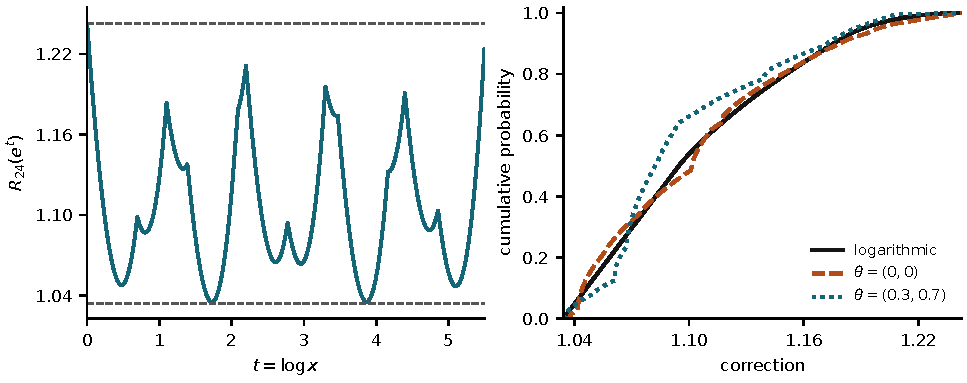
\includegraphics[width=\linewidth]{figures/laws.pdf}
\caption{The correction for $p=2$, $q=3$. Left, the solid curve is
$R_{24}(e^t)$ and the dashed lines mark its two limiting extrema.
Right, the logarithmic law and two integer subsequential laws from
\eqref{eq:natural}. Curves are deterministic quadrature approximations.}
\label{fig:laws}
\end{figure}
